%%%%%%%%%%%%%%%%%%%%%%% file tdp-draft.tex %%%%%%%%%%%%%%%%%%%%%%%%
%
% TDP Draft version 
% Created by Krit
%
%%%%%%%%%%%%%%%%%%%%%%%%%%%%%%%%%%%%%%%%%%%%%%%%%%%%%%%%%%%%%%%%%%%

\documentclass{llncs}

\usepackage{url}
\usepackage{amsmath}
\usepackage{array}
\usepackage{graphicx}

\newcommand{\dq}[1]{``#1''}
\newcommand{\dit}[1]{\dq{\textit{#1}}}
\newcommand{\md}[1]{\(#1\)}
\newcolumntype{C}[1]{>{\centering\let\newline\\\arraybackslash\hspace{0pt}}m{#1}}

\begin{document}

\title{SKUBA 2015 Team Description}
\author{Krit Chaiso
\and Jaktip Yodsri
\and Kandith Wongsuwan
\and Mukda Teeralertpanich
\and Konlayut Songkrasin \and Kanjanapan Sukvichai
}

\institute{ Faculty of Engineering, Kasetsart University\\
50 Ngamwongwan Rd, Ladyao, Bangkok, Thailand\\
\email{skuba2002@gmail.com}\\
\url{http://iml.cpe.ku.ac.th/skuba}
}

\maketitle

\begin{abstract}
This paper briefly describe software architecture and hardware design of SKUBA robot system, domestic service robot team from Kasetsart University, Thailand, in order to participate in Robocup@Home 2015. Our robot hardware doesn't have major change except the gripper that was redesigned in order to deal with object slippage that we encounter from previous Robocup. Robot wheels are redesigned in order to obtain the more precise motion. The research this year focus on data control system, deep learning for face detection, and furniture recognition which are our main problems from last year competition. This year, we'll evaluate our new techniques by using contest environment.
\end{abstract}

\section{Introduction}

SKUBA@home was established in 2011. In 2012, SKUBA@home made the first participation in Robocup Japan Open 2012 and made the way through finalist. Furthermore, SKUBA@home joined the World Robocup 2012 in Mexico and reach 2nd stage as we anticipated. We built the 2nd version robot in order to perform in the Robocup Japan Open 2013, Tokyo, and Robocup@home 2013, Eindhoven. In last year competition at Fukuoka, Robocup Japan Open 2014, we managed to archive the technical challenge reward.

In this year, we mainly emphasized on robot's perception. There are three major improvements on our robot's software components. First, face recognition module is reimplemented using deep learning approach, which is currently popular technique in machine learning area. Second, furniture recognition is purposed to enlarge the diversity of robot's perception. This component provide information about surrounding furniture, such as, tables and chairs. And, the final component is data control system which improves the effectiveness of perception as well as the development process. It handles the data storing and retrieving for other systems using database software.

The next section will explain about our robot mechanical, electrical design and calibration technique. In section 3, software architecture, face recognition with deep learning approach, methodology of furniture recognition and data control system are explained. Section 4 explains about controlling robot motion, such as, wheel and manipulator control. Finally in the last section, we will present the conclusion.

\section{Robot Hardware}

This year, the SKUBA@Home has been redesigned in order to improve the robot's hardware performance. We keep using three layers platform. The first layer, robot base layer, consists of four 6$''$ aluminum mecanum wheels. Because of robot motion issue, wheel vibration and annoying sound, therefore, the wheel's diameter is diminished from last year in order to make a robot achieve a precise movement, less mechanical slip and less vibrating sound. Each of them is driven by Maxon Brushless DC (BLDC) Motor combined with planetary gear-head of 1:36 gear ratio and FPGA embedded is chosen to be a main controller for 4 motors synchronously. The Hokuyo laser length finder (URG-04LX-UG01) is attached to the front of the base to gather surrounding information for navigation system.

The second layer is the robot arm and body. Last year, the measurement value of joint's angle was unreliable.  So, our arm's control system has been improved by using simple DC motor with an absolute encoder feedback, instead of using BLDC with potentiometer feedback. It helps to determine the joint angle, elbow and shoulder correctly and has more tolerate to noises. Two Dynamixel MX-28 servos and two High torque Dynamixel RX-64 servo are chosen to build a wrist and a gripper. Upgrading one of Dynamixel from RX-28 to MX-64 allows gripper to apply more force to make a tight grab. By combining all of actuator's motions, the arm can move freely in 6 degrees of freedom.

The final layer is robot head. The robot head has two degrees of freedom similar to human neck motion. R\O DE microphone, Kinect Sensor and Logitech C920 HD webcam are installed to Robot’s neck which can be used as anthropomorphic head. Due to low image quality of Kinect's RGB camera, HD webcam is substituted. To acquire the projection between webcam and Kinect axis, normal camera calibration algorithm does not work properly because of noisy depth data. Problem is solved by finding the transformation between webcam and Kinect's RGB first. Then it is biased with a constant distance value between depth sensor and Kinect's RGB camera which is much easier to do the calibration.

\begin{figure}
\centering
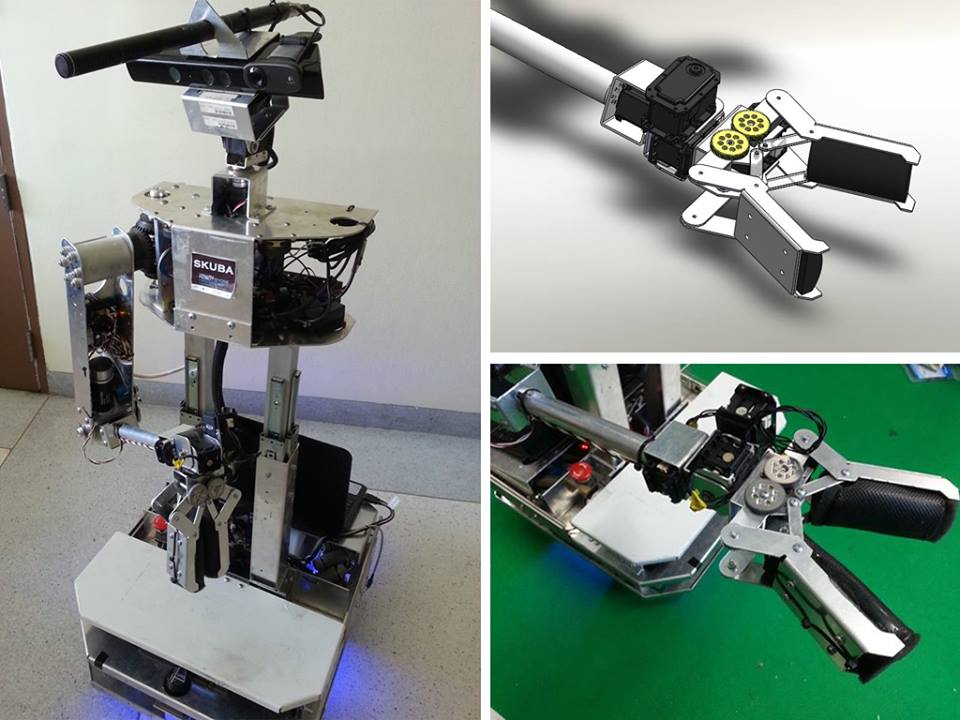
\includegraphics[height=6.2cm]{robot_hardware}
\caption{Robot hardware Left: The SKUBA@Home robot, Top Right: new gripper design, Bottom Right: actual gripper}
\label{fig:base}
\end{figure}

\section{Software Architecture}
Software system of our robot is divided into many modules with specific functionality, for example, object recognition module and planning module. The communication between modules is implemented by using Robot Operating System (ROS). The modules can be organized into three different layers:\textit{perception layer}, \textit{control layer} and \textit{decision layer}.

\textit{Perception layer} consist of modules about environmental understanding. Speech recognition, Object recognition and Localization, for instance. Modules in this layer collect various data from sensors, i.e., laser range finder, microphone and Kinect, to perform higher-level algorithms in order to identify states of the environment. The output of this layer is intermediate data for \textit{decision layer}

\textit{Decision layer} control robot's behavior to solve complicated task. In this layer, decision is made base on user command and information from perception layer. User command is classified into three categories: \textit{question}, \textit{command} and \textit{informative}. \textit{Question} is a sentence which user expect to get a proper answer from robot. \textit{Command} is used when user want robot to perform any action, for example, \dq{Bring me a pringle} and \dq{Follow me}. When robot get an information, such as \dq{My name is Brian} and \dq{This is kitchen}, these sentences will be classified as the \textit{Informative command}.

When \textit{decision layer} send command to robot, \textit{Control layer} will interpret those commands into lower-level actions by using path planning algorithms. Furthermore, the layer also controls robot manipulator with precision.

\subsection{Face Recognition}

Face recognition is basic ability for service robot to learn and classify human, such as, Serving meal and beverage. For this purpose, the robot has to memorize person who is the owner of the order. Due to complexity of the old face recognition algorithm, Elastic Bunch Graph Matching (EBGM), stacked spare autoencoder, deep learning technique, is used to solve this complexity. General stacked autoencoder is a neural network which contains two types of layers, autoencoder layer and logistic regression layer. Autoencoder layer is neural network with sparse constraint which transform data into feature space. And logistic regression layer is general neural network which classify the feature vector into a class.

In our face recognition system, stacked autoencoder is consist of one autoencoder layer and one logistic regression layer. There are two steps for training the stacked autoencoder, training autoencoder layer and logistic regression layer. To train autoencoder layer, Backpropagation with sparse penalty and regularization is used. By using input similar to target, this layer has to encode data into low dimension feature space and decode back to original dimension space. The other step is training logistic regression layer. Input of this step is product of autoencoder layer which is feature vector and target output is label of input data. General Backpropagation without any limitation is used to optimize logistic regression layer.

To visualize training result, the weight vectors of first autoencoder layer are extracted. Then reshape vector into images shown in Fig. \ref{fig:rec_face}. Extracted images are autoencoder recognized feature patterns for The ORL Database of Faces, taken by Cambridge University Computer Laboratory. Our algorithm is written in Theano library within GPU boosting\cite{theano_c1}\cite{theano_c2}.

\begin{figure}
\centering
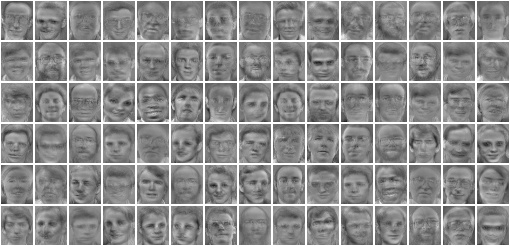
\includegraphics[height=5.2cm]{recognize_feature}
\caption{Images of recognize features.}
\label{fig:rec_face}
\end{figure} 

\subsection{Furniture Recognition System}

Furniture recognition is under the subset of object recognition focusing to perceive the existence of furniture. In order to recognize the furniture, Hough voting by using 3D point cloud is applied. First, the point cloud data obtained from Kinect is downsampled by using Uniform Sampling. Second, the Surface Normal Estimation is applied to let the surface normals be consistent with its surrounding. Next, in order to find descriptors, the key points and normals would be aggregated to form the 32 bins histogram. Then, the descriptor matching between the trained data and the given descriptor is performed by using KdTree with FLANN technique in order to find correspondences under a defined threshold. After getting the good matched descriptor, 3D Hough transform is used to cluster the groups of corresponding descriptors as well as to identify the object's category. Next, local Reference Frame and Iterative Closest Point algorithm are applied in order to obtain the precise position of the classified object.\cite{furniture}

\subsection{Data Control System}
In large-scale complexed system, the data management that is responsible for data retrieving and data storing  is one of the important component. Because of that, the method that uses database software to manage data is proposed. This component provides the data to the various modules such as trained image for object recognition, language structure for voice recognition or the positions of necessary location for navigation module. With this approach, the system can gain the well organized data as well as the effective data accessibility.


\subsection{Object Recognition}
    
To improve the precision of recognition module, localization approach is enhanced by using both RGB image and depth image together. First, depth information from OpenNI library is applied for extracting objects from the background scene using Euclidean Clustering Extraction\cite{rudu.thesis}. Additionally, there are some explicit constrains, e.g., table plane boundary and manipulator work space limitation, to distinguish the cloud that is definitely not the interested object, such as, the object that are beneath the table. After computing the centroid of extracted point cloud, object's border is transformed using the focal length equation from 3D space to RGB domain. From object's border, the segmented image is obtained. In image domain, descriptors of the segmented image are extracted using Speeded-Up Robust Features(SURF), and can be classified by a recognition process.

Another developed process is a recognition process. Initially, the extracted descriptors are clustered using K-means clustering. Next, the histogram for each object is created by counting the number of descriptors in each cluster. Finally, the set of histograms are used as learning instance for SVM method which is supervised learning for classification the object category\cite{obj_rec}.

The performance of this approach gains us the higher efficiency of both localization and recognition. First of all, localization using depth information has the acceptable accuracy for scoping the object boundary from the background scene. Lastly, recognition process has a significance of accuracy in classification comparing to our old method. Finally, result of this module is shown in Fig.\ref{fig:object_recog}.

\begin{figure}
\centering
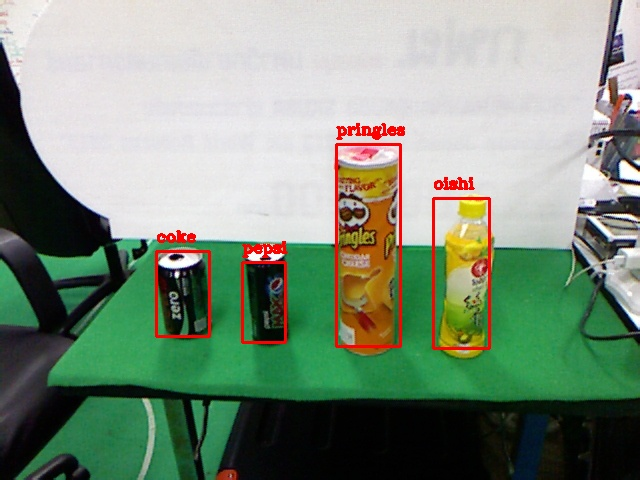
\includegraphics[height=6.2cm]{object_recognition_figure}
\caption{Result from object recognition module}
\label{fig:object_recog}
\end{figure}

\section{Motion Control and Planning}

\subsection{Motor Control System}

Control system is separated into two modules.The first module is base controller. Base controller uses FPGA embedded board to handle wheels. To operate the velocity of each wheel, the PI feedback controller is employed. The Hall sensors from every wheels are used to generate the feedback. And the communication between FPGA and computer is established by using RS232. The second module is arm controllers. Arm controllers use custom embedded board to handle DC motors for increase effort of arms. To manage its velocity and position, PID controller is employed. For precise movement, absolute encoders are used to read the arm position for apply in the PID Controller. The third module is a wrist motion controllers. For precise rotations, dynamixel servo motors are used. The connection between arm modules and computer are interacted within RS485.

\subsection{Localization and Path Planning}

Adaptive Monte Carlo Localization system (AMCL), provided by \textit{navigation} stack, is used for robot localization. To serve localization algorithm, Hokuyo laser length finder which acquires environmental data is attached to the robot. Additionally, the robot odometry information is also considered as one input information to localization algorithm. Another input is the known map, shown in Fig.\ref{fig:hector}, which is statically or dynamically construct. From previously describe input, AMCL which is a particle filter localization system accurately estimates position and orientation of the robot.

\begin{figure}
\centering
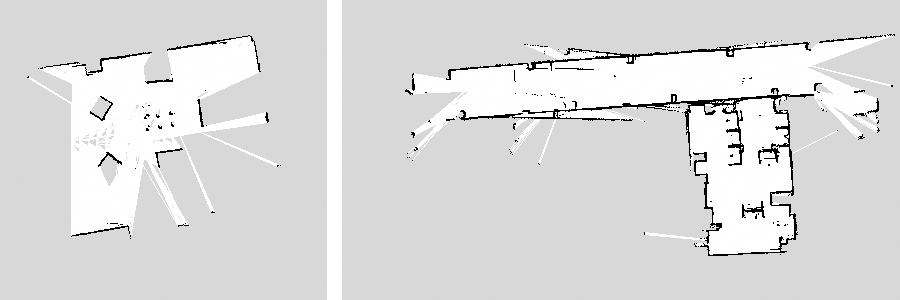
\includegraphics[height=3.9cm]{hector_map}
\caption{Occupancy map from \textit{hector\_mapping}}
\label{fig:hector}
\end{figure}

To achieve path planning, there is \textit{move\_base} node in \textit{navigation} stack that is consist of two types of planning method. Begin with global planner, this method provides an effective path for robot to navigate through the known map. By using Dijkstra's algorithm, the result path is the shortest and acceptable. Then local planner method move to destination following designated path and avoid obstacles along the way. In order to move robot, local planner determine its velocity and orientation. This node directly send command to the robot.

\subsubsection{Odometry Estimation Module}

This module helps to minimize the mean square error of the non-perfect sensor measurement originated from wheel slippage, dynamic surrounded environment and IMU drift over time. Using the laser scanner to estimate the change of position by laser scan matching technique can solve the wheel slip problem while facing with high sensitivity and dynamic environment. Point-to-line distance Iterative Closed Point (ICP) method is used to be based algorithm for laser scan matching.

To perform estimation module, Kalman filter which consist of two steps is used. First, the Kalman's observation step calculates difference between output from last prediction and actual position which combine laser scan matching and wheels' speed together. Next, the Kalman's prediction step predicts new output by compensate error from previous step and IMU data\cite{odom}.

\subsubsection{Collision Avoidance Module}

This component ease the planning module to organize safety movement. By retrieve point cloud data from Kinect, this module projects each point to occupancy map. In order to avoid obstacles, path planner retrieve projection data and manage to construct smooth path. Due to unusual data, such as, ground plane and wall partition, planar elimination algorithm is applied. Result data from algorithm, for instance, table and chair, is projected and pass to planning module continuously\cite{avoid}.

\subsection{Manipulation Module}

For the manipulation system, two distinct methods are developed for serving various situation. First, grasping action method uses a shape of particular object as input. And it selects appropriate movement from predefine sequences of action and send command to robot arm. In generally, this method use for object which has a complicated shape. Another method is inverse kinematic method that receive the centroid of an object and directly control robot's manipulator. So, this method use with a simple object, e.g., can, box and bottle.

\section{Conclusion}

In this year, perception and manipulation are our main focuses. Data control system, deep learning for face detection, and furniture recognition are our main focuses for our software system's improvement. Robot hardware had been modified and redesigned in order to achieve a superior performance by encountering the hardware parts that cause the robot motion and manipulator issues. We gained experiences from RoboCup@Home Japan Open competition 2014 and discovered development idea. For Robocup@Home 2015 in China, our robot are more autonomous and ready for engage in competition. We hope that our robot team will perform better in RoboCup than the previous year, and we are looking forward to sharing experiences with other great teams around the world.

\section*{Team Member}

This year, SKUBA@home team is consist of this following members:
\begin{itemize}
\item Supervisor: Kanjanapan Sukvichai
\item Team Leader: Kandith Wongsuwan
\item Computer Engineering: Krit Chaiso, Jaktip Yodsri, Phatthawipha Jeamburanakul, Mukda Teeralertpanich, Nut Kaewnak, Udom Chaowanakosol, Thanakorn Panyapiang, Tachin Srisombat, and Tisana Kitsahawong
\item Electrical Engineering: Konlayut Songkrasin, Pasuk Yodpanun, Teeratath Ariyachartphadungkit, Suppawit Inhorm, and Patcharapon Pimpa
\item Mechanical Engineering: Tanakrit Techadejworaphun, Vasuwat Kittiwangchai, and Sutinai Tanalerkchai
\end{itemize}
\begin{thebibliography}{4}

\bibitem{con_arm} T. Ariyachartphadungkit and K. Sukvichai, Development of an Embedded BLDC motor controller using RS485 standard, 2013.

\bibitem{theano_c1}F. Bastien, P. Lamblin, R. Pascanu, J. Bergstra, I. Goodfellow, A. Bergeron, N. Bouchard, D. Warde-Farley and Y. Bengio. Theano: new features and speed improvements. NIPS 2012 deep learning workshop.

\bibitem{theano_c2}J. Bergstra, O. Breuleux, F. Bastien, P. Lamblin, R. Pascanu, G. Desjardins, J. Turian, D. Warde-Farley and Y. Bengio. Theano: A CPU and GPU Math Expression Compiler. Proceedings of the Python for Scientific Computing Conference (SciPy) 2010. June 30 - July 3, Austin, TX

\bibitem{furniture}F. Tombari and L. Di Stefano, Object recognition in 3D scenes with occlusions and clutter by Hough voting, 4th Pacific-Rim Symposium on Image and Video Technology, 2010.

\bibitem{rudu.thesis} Radu B. Rusu, 
Semantic 3D Object Maps for Everyday Manipulation in Human Living Environments, Germany, 2009.

\bibitem{obj_rec} D. Schmitt and N. McCoy. Object Classification and Localization Using SURF Descriptors. 2011.

\bibitem{face_reg} L. Wiskott, J.M. Fellous, N. Kruger and C. Malsburg, Face Recognition by Elastic Bunch Graph Matching, IEEE Trans. PAMI, vol. 19, no. 7, pp. 775-780, 1997. 

\bibitem{pp_detect} M. Munaro, F. Basso and E. Menegatti. Tracking people within groups with RGB-D data. In Proceedings of the International Conference on Intelligent Robots and Systems (IROS) 2012, Vilamoura (Portugal), 2012.

\bibitem{hector_slam} S. Kohlbrecher and J. Meyer and O. von Stryk and U. Klingauf. A Flexible and Scalable SLAM System with Full 3D Motion Estimation, in Proc. IEEE International Symposium on Safety, Security and Rescue Robotics (SSRR), November, 2011.

\bibitem{odom} B. Pholpoke and K. Sukvichai. Real Time People Tracking and Collision Avoidance using Sensors Fusion for an Indoor Omni-directional Wheels Mobile Robot, 2013.

\bibitem{avoid} T. Chaveekolakit and K. Sukvichai. Development of Ground Planar Segmentation algorithm using 3D Point Clouds Information from Kinect Depth Image Camera, 2013.

\end{thebibliography}

\end{document}
